\section{Results}

\subsection{Phase transitions}

The results (\cref{fig:phase}) indicated a phase transitions for T $\in
\brak{2.2,2.35}$. The simulations with higher grid size exhibits sharper
changes, meaning that they will capture the phase transition better, because of
a smaller contribution from the boundaries.

\begin{figure}[ht]
  \centering
  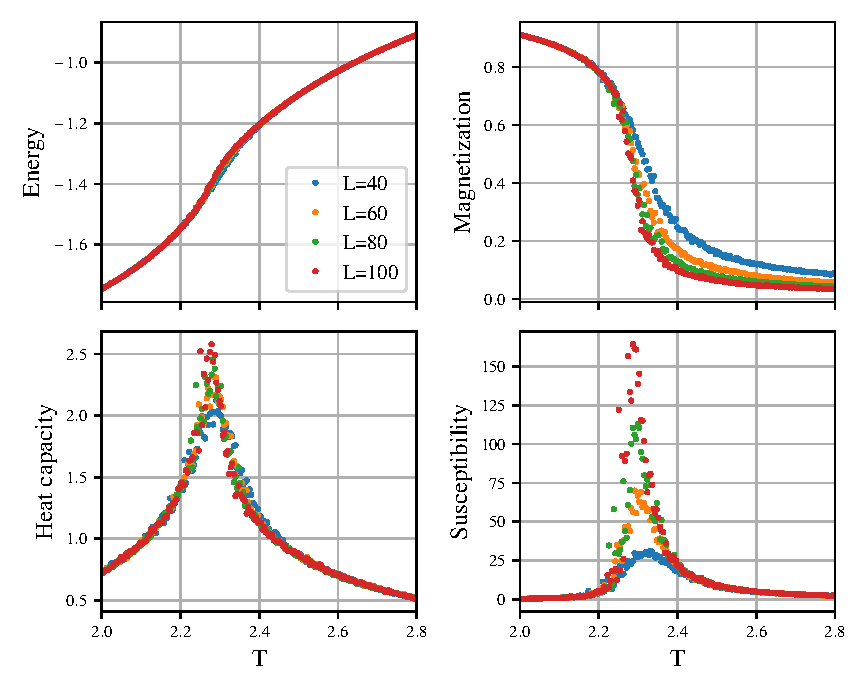
\includegraphics[width=\textwidth]{../figures/phase.pdf}
  \caption{Simulating for various temperatures looking for phase transitions.\\
  T $\in \brak{2.0,2.8}$, dT = \num{4e-3}, \num{1e6} MC cycles, delay=50000}
  \label{fig:phase}
\end{figure}


To better capture the peaks of $C_v$ and $\chi$ we did another
run with dT = \num{5e-4} for T $\in \brak{2.2, 2.35}$.
 We fitted sixth order polynomials to $C_v$ and found
the critical temperature Tc$_{L}$ for each grid size (\ref{fig:polyfit}).


\begin{equation}
  \label{eq:scaling}
  T_C(L=\infty) = T_C(L) - aL^{-1/\nu}
\end{equation}

Using the finite size scaling relation in
\cref{eq:scaling} with $\nu$ = 1, we estimated $T_c(L=\infty)$
by doing a linear
regression with the four different T$_C$(L), using $1/L$ as the independent
variable, and extracting the intercept (\cref{fig:lin_reg}).
\footnote{Implemented in critical\_temperature.py}.  This gave us the result of $T_C=2.2687$, with absolute and relative error
 given in \cref{tab:critical}.




 \begin{figure}[ht]
   \begin{subfigure}[t]{.5\textwidth} % top align
     \centering
     % include first image
     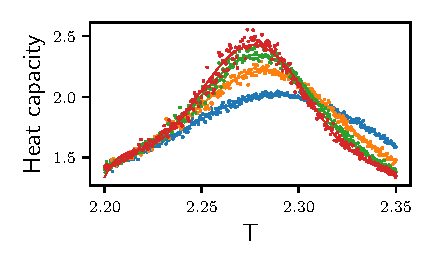
\includegraphics[width=\linewidth]{../figures/fit.pdf}
     \caption{Fit of sixth order polynomials (lines) to the measurements
     of heat capacity (circles).}
     \label{fig:polyfit}
   \end{subfigure}
   \hfill
   \begin{subfigure}[t]{.5\textwidth}
     \centering
     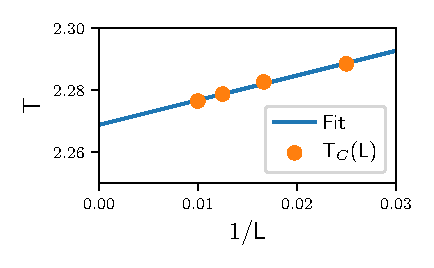
\includegraphics[width=\linewidth]{../figures/Tc_fit.pdf}
     \caption{Linear regression on the critical temperatures for L $\in \brak{[40,60,80,100]}$
     to extrapolate T$_C(L=\infty)$.}
     \label{fig:lin_reg}
   \end{subfigure}
   \label{fig:test}
 \end{figure}




 \begin{table}[htp]
   \centering
   \csvautotabular{../data/critical.csv}
   \caption{Results for T$_C(L=\infty)$.}
   \label{tab:critical}
 \end{table}
